\chapter{Manipulació de bits}

Totes les dades dels programes informàtics s'emmagatzemen internament
com a bits, és a dir, com a números 0 i 1. En aquest capítol es parla
de la representació binària dels nombres enters i mostra exemples de
com utilitzar operacions de bits. Resulta que hi ha molts usos per a
la manipulació de bits en la programació d'algorismes.

\section{Representació binària}

\index{representació binària}

Quan programem, els enters de $n$ bits s'emmagatzemen internament com
a nombres binaris de $n$ bits. Per exemple, el tipus C++ \texttt{int}
és un tipus de 32 bits, i cada nombre \texttt{int} es representa amb
32 bits.

Aquí teniu la representació binària del nombre de tipus \texttt{int} 43:
\[00000000000000000000000000101011\]
Els bits de la representació s'indexen de dreta a esquerra. Per
convertir una representació binària $b_k \cdots b_2 b_1 b_0$ en un
nombre, podem fer servir la fórmula
\[b_k 2^k + \ldots + b_2 2^2 + b_1 2^1 + b_0 2^0.\]
Per exemple,
\[1 \cdot 2^5 + 1 \cdot 2^3 + 1 \cdot 2^1 + 1 \cdot 2^0 = 43.\]


La representació binària d'un nombre és \key{amb signe}
(\emph{signed}) o \key{sense signe} (\emph{unsigned}). Normalment
s'utilitza una representació amb signe, el que significa que es poden
representar tant nombres negatius com positius. Una variable amb signe
de $n$ bits pot contenir qualsevol nombre enter entre $-2^{n-1}$ i
$2^{n-1}-1$. Per exemple, el tipus \texttt{int} en C++ és un tipus
signat, de manera que una variable \texttt{int} pot contenir qualsevol
nombre enter entre $-2^{31}$ i $2^{31}-1$.

El primer bit d'una representació amb signe és el signe del nombre (0
per a nombres no negatius i 1 per a nombres negatius), i els $n-1$
restants contenen la magnitud del nombre. S'utilitza \key{Complement
  de dos}, que significa que el nombre oposat d'un nombre es calcula
invertint primer tots els bits del nombre i després augmentant el
nombre en un.

Per exemple, la representació binària del nombre \texttt{int} $-43$ és
\[11111111111111111111111111010101.\]


En una representació sense signe, només es poden fer servir nombres no
negatius, però el límit superior dels valors és més gran. Una variable
sense signe de $n$ bits pot contenir qualsevol nombre enter entre $0$
i $2^n-1$. Per exemple, en C++, una variable \texttt{unsigned int} pot
contenir qualsevol nombre enter entre $0$ i $2^{32}-1$.

Hi ha una connexió entre les representacions: un nombre amb signe $-x$ és
igual a un nombre sense signe $2^n-x$. Per exemple, el codi següent
mostra que el número amb signe $x=-43$ és igual al nombre sense signe
$y=2^{32}-43$:
\begin{lstlisting}
int x = -43;
unsigned int y = x;
cout << x << "\n"; // -43
cout << y << "\n"; // 4294967253
\end{lstlisting}


Si un nombre és més gran que el límit superior de la representació de
bits, el nombre es desbordarà. En una representació amb signe, el
nombre que segueix $2^{n-1}-1$ és $-2^{n-1}$, i en una representació
sense signe, el nombre que segueix $2^n-1$ és $0$\footnote{(N. del T.)
En C++, està permès fer operacions aritmètiques que causin
\emph{overflow} en tipus sense signe, però fer-ho amb tipus amb signe
és comportament no definit (\emph{undefined behavior}). No és un
problema dels processadors, que poden fer \emph{overflow} de nombres
amb signe sense problema, sinó dels compiladors de C++, que optimitzen
el codi agressivament sota el supòsit que el vostre programa mai comet
\emph{undefined behavior}. No ho feu.}. Per exemple, considereu el
codi següent:
\begin{lstlisting}
int x = 2147483647
cout << x << "\n"; // 2147483647
x++;
cout << x << "\n"; // -2147483648
\end{lstlisting}

Inicialment, el valor de $x$ és $2^{31}-1$. Aquest és el valor més
gran que es pot emmagatzemar en una variable \texttt{int}, de manera
que el nombre següent després de $2^{31}-1$ és $-2^{31}$.



\section{Operacions de bits}

\newcommand\XOR{\mathbin{\char`\^}}

\subsubsection{Operació \emph{and}}

\index{operació and}

L'operació \key{\emph{and}} $x$ \& $y$ produeix un nombre que té un
bit en les posicions on tant $x$ com $y$ tenen un bit. Per exemple, $22$
\& $26$ = 18, perquè


\begin{center}
\begin{tabular}{rrr}
& 10110 & (22)\\
\& & 11010 & (26) \\
\hline
 = & 10010 & (18) \\
\end{tabular}
\end{center}


Mitjançant l'operació (\emph{and}), podem comprovar si un nombre
$x$ és parell perquè $x$ \& $1$ = 0 si $x$ és parell, i $x$ \& $1$ = 1
si $x$ és senar. De manera més general, $x$ és divisible per $2^k$
exactament quan $x$ \& $(2^k-1)$ = 0.

\subsubsection{Operació \emph{or}}

\index{operació or}

L'operació \key{\emph{OR}} $x$ | $y$ produeix un nombre que té un bit
en les posicions on $x$ o $y$ tenen un bit. Per exemple, $22$ |
$26$ = 30, perquè


\begin{center}
\begin{tabular}{rrr}
& 10110 & (22)\\
| & 11010 & (26) \\
\hline
 = & 11110 & (30) \\
\end{tabular}
\end{center}


\subsubsection{Operació \emph{xor}}

\index{operació xor}

L'operació \key{xor} $x$ $\XOR$ $y$ produeix un nombre que té un bit
en les posicions on exactament un de $x$ i $y$ tenen un bit. Per exemple,
$22$ $\XOR$ $26$ = 12, perquè


\begin{center}
\begin{tabular}{rrr}
& 10110 & (22)\\
$\XOR$ & 11010 & (26) \\
\hline
 = & 01100 & (12) \\
\end{tabular}
\end{center}


\subsubsection{Operació \emph{not}}

\index{Operació not}

L'operació \key{\emph{not}} \textasciitilde$x$ produeix un nombre on tots els
bits de $x$ s'han invertit. En complement a 2 es compleix que
\textasciitilde$x = -x-1$. Per exemple, \textasciitilde$29 = -30$.

El resultat de l'operació \emph{not} a nivell de bits depèn de la
longitud de la representació binària, perquè l'operació inverteix tots
els bits. Per exemple, si els nombres són \emph{int}s de 32 bits, el
resultat és el següent:


\begin{center}
\begin{tabular}{rrrr}
$x$ & = & 29 &   00000000000000000000000000011101 \\
\textasciitilde$x$ & = & $-30$ & 11111111111111111111111111100010 \\
\end{tabular}
\end{center}


\subsubsection{Desplaçament de bits}

\index{desplaçament de bits}

El desplaçament de bits (\emph{bit shift}) a l'esquerra $x < < k$
afegeix $k$ bits zero al nombre, i el desplaçament de bits a la dreta
$x > > k$ elimina els darrers $k$ bits del nombre. Per exemple, $14 < <
2 = 56$, perquè $14$ i $56$ són 1110 i 111000 en binari. De la mateixa
manera, $49 > > 3 = 6$, perquè $49$ i $6$ són 110001 i 110.

Tingueu en compte que $x < < k$ correspon a multiplicar $x$ per $2^k$,
i $x > > k$ correspon a dividir $x$ per $2^k$ arrodonint a un nombre
enter.

\subsubsection{Aplicacions}

Un nombre de la forma $1 < < k$ té un bit a la posició $k$ i tots els
altres bits són zero, de manera que podem fem servir aquests nombres
per accedir als bits individuals d'un nombre donat. En particular, el
$k$-èsim bit d'un nombre és 1 exactament quan $x$ \& $(1 < < k)$ no
és zero. El codi següent imprimeix la representació binària d'un
nombre $x$ de tipus \texttt{int}:


\begin{lstlisting}
for (int i = 31; i >= 0; i--) {
    if (x&(1<<i)) cout << "1";
    else cout << "0";
}
\end{lstlisting}


També és possible modificar bits individuals fent servir idees
similars. Per exemple, la fórmula $x$ | $(1 < < k)$ posa el $k$-èsim
bit de $x$ a 1, la fórmula $x$ \& \textasciitilde $(1 < < k)$ posa el
$k$-èsim bit de $x$ a 0, i la fórmula $x$ $\XOR$ $(1 < < k)$
inverteix el $k$-èsim bit de $x$.

La fórmula $x$ \& $(x-1)$ posa l'últim bit de $x$ a zero, i la fórmula
$x$ \& $-x$ posa tots els bits a zero, excepte l'últim. La
fórmula $x$ | $(x-1)$ inverteix tots els bits després de l'últim
bit. Tingueu en compte també que un nombre positiu $x$ és una potència
de dos exactament quan $x$ \& $(x-1) = 0$.

\subsubsection*{Funcions addicionals}

El compilador g++ proporciona les funcions següents per comptar bits:


\begin{itemize}
\item
$\texttt{\_\_builtin\_clz}(x)$:
the number of zeros at the beginning of the number
\item
$\texttt{\_\_builtin\_ctz}(x)$:
the number of zeros at the end of the number
\item
$\texttt{\_\_builtin\_popcount}(x)$:
the number of ones in the number
\item
$\texttt{\_\_builtin\_parity}(x)$:
the parity (even or odd) of the number of ones
\end{itemize}

\begin{samepage}

The functions can be used as follows:
\begin{lstlisting}
int x = 5328; // 00000000000000000001010011010000
cout << __builtin_clz(x) << "\n"; // 19
cout << __builtin_ctz(x) << "\n"; // 4
cout << __builtin_popcount(x) << "\n"; // 5
cout << __builtin_parity(x) << "\n"; // 1
\end{lstlisting}
\end{samepage}


Tot i que les funcions anteriors només admeten nombres de tipus
\texttt{int}, també hi ha versions \texttt{longlong} de les funcions
amb el sufix \texttt{ll}.

\section{Representació de conjunts}

Cada subconjunt d'un conjunt $\{0,1,2,\ldots,n-1\}$ es pot representar
com un nombre enter de $n$ bits els bits del qual indiquen quins
elements pertanyen al subconjunt. Aquesta és una manera eficient de
representar conjunts, perquè cada element només requereix un bit de
memòria i les operacions de conjunt es poden implementar com a
operacions de bits.

Per exemple, com que \texttt{int} és un tipus de 32 bits, un nombre
\texttt{int} pot representar qualsevol subconjunt del conjunt
$\{0,1,2,\ldots,31\}$. La representació binària del conjunt
$\{1,3,4,8\}$ és
\[00000000000000000000000100011010,\]
que correspon al nombre $2^8+2^4+2^3+2^1=282$.

\subsubsection{Implementació de conjunts}

El codi següent declara una variable \texttt{int} $x$ que pot contenir
un subconjunt de $\{0,1,2,\ldots,31\}$. Després d'això, el codi
afegeix els elements 1, 3, 4 i 8 al conjunt i imprimeix la seva mida.
\begin{lstlisting}
int x = 0;
x |= (1<<1);
x |= (1<<3);
x |= (1<<4);
x |= (1<<8);
cout << __builtin_popcount(x) << "\n"; // 4
\end{lstlisting}
El codi següent imprimeix tots els elements que pertanyen al conjunt:
\begin{lstlisting}
for (int i = 0; i < 32; i++) {
    if (x&(1<<i)) cout << i << " ";
}
// output: 1 3 4 8
\end{lstlisting}


\subsubsection{Operacions de conjunts}

Les operacions de conjunt es poden implementar de la següent manera
com a operacions de bits:


\begin{center}
\begin{tabular}{lll}
& set syntax & bit syntax \\
\hline
intersection & $a \cap b$ & $a$ \& $b$ \\
union & $a \cup b$ & $a$ | $b$ \\
complement & $\bar a$ & \textasciitilde$a$ \\
difference & $a \setminus b$ & $a$ \& (\textasciitilde$b$) \\
\end{tabular}
\end{center}


Per exemple, el codi següent construeix primer els conjunts
$x=\{1,3,4,8\}$ i $y=\{3,6,8,9\}$, i després construeix el conjunt $z
= x \cup y = \{1,3,4,6,8,9\}$:


\begin{lstlisting}
int x = (1<<1)|(1<<3)|(1<<4)|(1<<8);
int y = (1<<3)|(1<<6)|(1<<8)|(1<<9);
int z = x|y;
cout << __builtin_popcount(z) << "\n"; // 6
\end{lstlisting}


\subsubsection{Iteració de subconjunts}

El codi següent passa per tots els subconjunts de
$\{0,1,\ldots,n-1\}$:


\begin{lstlisting}
for (int b = 0; b < (1<<n); b++) {
    // process subset b
}
\end{lstlisting}
El codi següent passa pels subconjunts amb exactament $k$ elements:
\begin{lstlisting}
for (int b = 0; b < (1<<n); b++) {
    if (__builtin_popcount(b) == k) {
        // process subset b
    }
}
\end{lstlisting}
El codi següent passa pels subconjunts d'un conjunt $x$:
\begin{lstlisting}
int b = 0;
do {
    // process subset b
} while (b=(b-x)&x);
\end{lstlisting}


\section{Optimitzacions de bits}

Molts algorismes es poden optimitzar mitjançant operacions de
bits. Aquestes optimitzacions no canvien la complexitat temporal de
l'algorisme, però poden tenir un gran impacte en el temps real
d'execució del codi. En aquesta secció comentem exemples d'aquestes
situacions.

\subsubsection{Distàncies de Hamming}

\index{Distància de Hamming} La \key{distància de Hamming}
$\texttt{hamming}(a,b)$ entre dues cadenes $a$ i $b$ d'igual longitud
és el nombre de posicions on les cadenes difereixen. Per exemple,
\[\texttt{hamming}(01101,11001)=2.\]


Considereu el problema següent: donada una llista de $n$ cadenes de
bits, cadascuna de longitud $k$, calculeu la distància de Hamming
mínima entre dues cadenes de la llista. Per exemple, la resposta per a
$[00111,01101,11110]$ és 2, perquè
\begin{itemize}[noitemsep]
\item $\texttt{hamming}(00111,01101)=2$,
\item $\texttt{ hamming}(00111,11110)=3$ i
\item $\texttt{hamming}(01101,11110)=3$.
\end{itemize}

Una manera senzilla de resoldre el problema és passar per tots els
parells de cordes i calcular les seves distàncies de Hamming, que dóna
lloc a un algorisme de temps $O(n^2 k)$. La funció següent es pot
utilitzar per calcular distàncies:
\begin{lstlisting}
int hamming(string a, string b) {
    int d = 0;
    for (int i = 0; i < k; i++) {
        if (a[i] != b[i]) d++;
    }
    return d;
}
\end{lstlisting}


Tanmateix, si $k$ és petit, podem optimitzar el codi emmagatzemant les
cadenes binàries com a nombres enters i calculant les distàncies de
Hamming mitjançant operacions de bits. En particular, si $k \le 32$,
podem simplement emmagatzemar les cadenes com a valors \texttt{int} i
utilitzar la funció següent per calcular distàncies:
\begin{lstlisting}
int hamming(int a, int b) {
    return __builtin_popcount(a^b);
}
\end{lstlisting}
A la funció anterior, l'operació \emph{xor} construeix una cadena binària que
té un bit en posicions on $a$ i $b$ difereixen, i a continuació calculem
el nombre de bits mitjançant la funció \texttt{\_\_builtin\_popcount}.

Per a comparar les implementacions, generem una llista de 10.000
cadenes binàries aleatòries de longitud 30. Amb el primer enfocament, la
cerca triga $13.5$ segons, però si fem servir l'optimització de bits,
només triga $0.5$ segons. El codi optimitzat per bits és gairebé 30
vegades més ràpid que el codi original.

\subsubsection{Comptar subquadrícules}

Com a altre exemple, considereu el problema següent: Donada una
quadrícula $n \times n$ cada quadrat de la qual és negre (1) o blanc
(0), calculeu el nombre de subquadrícules que tenen totes les
cantonades negres. Per exemple, la quadrícula
\begin{center}
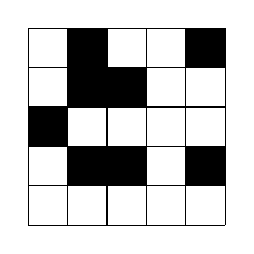
\begin{tikzpicture}[scale=0.5]
\fill[black] (1,1) rectangle (2,2);
\fill[black] (1,4) rectangle (2,5);
\fill[black] (4,1) rectangle (5,2);
\fill[black] (4,4) rectangle (5,5);
\fill[black] (1,3) rectangle (2,4);
\fill[black] (2,3) rectangle (3,4);
\fill[black] (2,1) rectangle (3,2);
\fill[black] (0,2) rectangle (1,3);
\draw (0,0) grid (5,5);
\end{tikzpicture}
\end{center}
conté dues subquadrícules d'aquest tipus:
\begin{center}
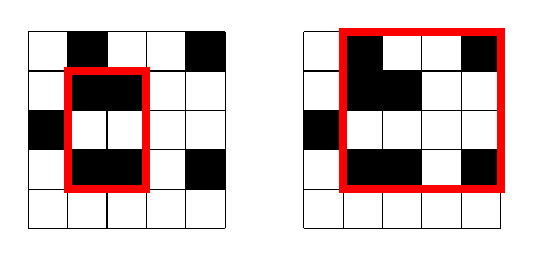
\begin{tikzpicture}[scale=0.5]
\fill[black] (1,1) rectangle (2,2);
\fill[black] (1,4) rectangle (2,5);
\fill[black] (4,1) rectangle (5,2);
\fill[black] (4,4) rectangle (5,5);
\fill[black] (1,3) rectangle (2,4);
\fill[black] (2,3) rectangle (3,4);
\fill[black] (2,1) rectangle (3,2);
\fill[black] (0,2) rectangle (1,3);
\draw (0,0) grid (5,5);

\fill[black] (7+1,1) rectangle (7+2,2);
\fill[black] (7+1,4) rectangle (7+2,5);
\fill[black] (7+4,1) rectangle (7+5,2);
\fill[black] (7+4,4) rectangle (7+5,5);
\fill[black] (7+1,3) rectangle (7+2,4);
\fill[black] (7+2,3) rectangle (7+3,4);
\fill[black] (7+2,1) rectangle (7+3,2);
\fill[black] (7+0,2) rectangle (7+1,3);
\draw (7+0,0) grid (7+5,5);

\draw[color=red,line width=1mm] (1,1) rectangle (3,4);
\draw[color=red,line width=1mm] (7+1,1) rectangle (7+5,5);
\end{tikzpicture}
\end{center}


Hi ha un algorisme de temps $O(n^3)$ que resol el problema: passeu
per tots els parells de files $O(n^2)$ i per a cada parell $(a,b)$
calculeu el nombre de columnes que contenen un quadrat negre a les
dues files en $O(n)$ temps. El codi següent assumeix que
$\texttt{color}[y][x]$ denota el color de la fila $y$ i la columna $x$:
\begin{lstlisting}
int count = 0;
for (int i = 0; i < n; i++) {
    if (color[a][i] == 1 && color[b][i] == 1) count++;
}
\end{lstlisting}
Aleshores, aquestes columnes representen subquadrícules
$\texttt{count}(\texttt{count}-1)/2$ amb cantonades negres, perquè
podem triar-ne dues per formar una subquadrícula.

Per optimitzar aquest algorisme, dividim la cuadrícula en blocs de
columnes de manera que cada bloc consta de $N$ columnes
consecutives. Aleshores, cada fila s'emmagatzema com una llista de
números de $N$ bits que descriuen els colors dels quadrats. Ara podem
processar $N$ columnes simultàniament gràcies a les operacions de
bits. Al codi següent, $\texttt{color}[y][k]$ representa un bloc de
$N$ colors com a bits.
\begin{lstlisting}
int count = 0;
for (int i = 0; i <= n/N; i++) {
    count += __builtin_popcount(color[a][i]&color[b][i]);
}
\end{lstlisting}
L'algorisme resultant funciona en temps $O(n^3/N)$.

Generem una graella aleatòria de $2500 \times 2500$ i comparem la
implementació original i la implementació optimitzada per bits. El
codi original triga $29.6$ segons, mentre que la versió optimitzada
per bits només triga $3.1$ segons amb $N=32$ (nombres
\texttt{int}) i $1.7$ segons amb $N=64$ (nombres \texttt{longlong}).

\section{Programació dinàmica}
\label{bits-dp}

Les operacions de bits proporcionen una manera eficient i còmoda
d'implementar algorismes de programació dinàmica els estats dels quals
contenen subconjunts d'elements, perquè aquests estats es poden
emmagatzemar com a nombres enters. A continuació discutim exemples de
combinació d'operacions de bits i programació dinàmica.

\subsubsection{Selecció òptima}

Com a primer exemple, considereu el problema següent: Ens donen els
preus de $k$ productes durant $n$ dies i volem comprar cada producte
exactament una vegada. Tanmateix, podem comprar com a màxim un
producte al dia. Quin és el preu total mínim? Per exemple, considereu
l'escenari següent ($k=3$ i $n=8$):
\begin{center}
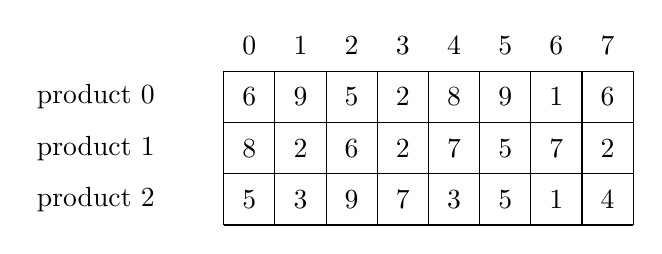
\begin{tikzpicture}[scale=.65]
    \draw (0, 0) grid (8,3);
    \node at (-2.5,2.5) {product 0};
    \node at (-2.5,1.5) {product 1};
    \node at (-2.5,0.5) {product 2};

    \foreach \x in {0,...,7}
        {\node at (\x+0.5,3.5) {\x};}
    \foreach \x/\v in {0/6,1/9,2/5,3/2,4/8,5/9,6/1,7/6}
        {\node at (\x+0.5,2.5) {\v};}
    \foreach \x/\v in {0/8,1/2,2/6,3/2,4/7,5/5,6/7,7/2}
        {\node at (\x+0.5,1.5) {\v};}
    \foreach \x/\v in {0/5,1/3,2/9,3/7,4/3,5/5,6/1,7/4}
        {\node at (\x+0.5,0.5) {\v};}
\end{tikzpicture}
\end{center}
En aquest escenari, el preu total mínim és de $5$:
\begin{center}
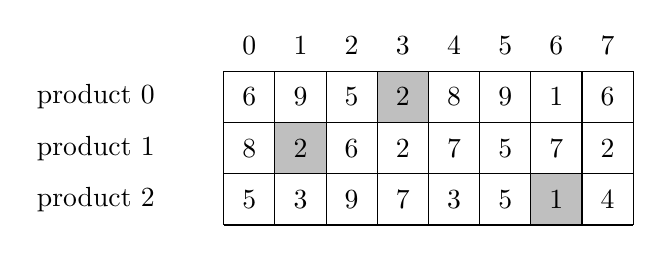
\begin{tikzpicture}[scale=.65]
    \fill [color=lightgray] (1, 1) rectangle (2, 2);
    \fill [color=lightgray] (3, 2) rectangle (4, 3);
    \fill [color=lightgray] (6, 0) rectangle (7, 1);
    \draw (0, 0) grid (8,3);
    \node at (-2.5,2.5) {product 0};
    \node at (-2.5,1.5) {product 1};
    \node at (-2.5,0.5) {product 2};

    \foreach \x in {0,...,7}
        {\node at (\x+0.5,3.5) {\x};}
    \foreach \x/\v in {0/6,1/9,2/5,3/2,4/8,5/9,6/1,7/6}
        {\node at (\x+0.5,2.5) {\v};}
    \foreach \x/\v in {0/8,1/2,2/6,3/2,4/7,5/5,6/7,7/2}
        {\node at (\x+0.5,1.5) {\v};}
    \foreach \x/\v in {0/5,1/3,2/9,3/7,4/3,5/5,6/1,7/4}
        {\node at (\x+0.5,0.5) {\v};}
\end{tikzpicture}
\end{center}


Sigui $\texttt{price}[x][d]$ el preu del producte $x$ el dia $d$. Per
exemple, a l'escenari anterior $\texttt{price}[2][3] = 7$. Sigui
$\texttt{total}(S,d)$ el preu total mínim per
comprar un subconjunt $S$ de productes en els primers $d$ dies. Amb aquesta
funció, la solució al problema és $\texttt{total}(\{0 \ldots
k-1\},n-1)$.

Primer, $\texttt{total}(\emptyset,d) = 0$, perquè no costa res comprar
un conjunt buit, i $\texttt{total}(\{x\},0) = \texttt{price}[x][0]$,
perquè hi ha una manera de comprar un producte el primer
dia. Aleshores, es pot utilitzar la recurrència següent:
\begin{equation*}
\begin{split}
\texttt{total}(S,d) = \min( & \texttt{total}(S,d-1), \\
& \min_{x \in S} (\texttt{total}(S \setminus x,d-1)+\texttt{price}[x][d]))
\end{split}
\end{equation*}
Això vol dir que o bé no comprem cap producte el dia $d$ o bé comprem un
producte $x$ que pertany a $S$. En aquest últim cas, eliminem $x$ de
$S$ i afegim el preu de $x$ al preu total.

El següent pas és calcular els valors de la funció mitjançant la
programació dinàmica. Per emmagatzemar els valors de la funció,
declarem una matriu
\begin{lstlisting}
int total[1<<K][N];
\end{lstlisting}
on $K$ i $N$ són constants adequadament grans.  La primera dimensió de
la matriu correspon a una representació de bits d'un subconjunt.

En primer lloc, els casos en què $d=0$ es poden processar de la
següent manera:
\begin{lstlisting}
for (int x = 0; x < k; x++) {
    total[1<<x][0] = price[x][0];
}
\end{lstlisting}
Aleshores, la recurrència es tradueix al codi següent:
\begin{lstlisting}
for (int d = 1; d < n; d++) {
    for (int s = 0; s < (1<<k); s++) {
        total[s][d] = total[s][d-1];
        for (int x = 0; x < k; x++) {
            if (s&(1<<x)) {
                total[s][d] = min(total[s][d],
                                    total[s^(1<<x)][d-1]+price[x][d]);
            }
        }
    }
}
\end{lstlisting}
La complexitat temporal de l'algorisme és $O(n 2^k k)$.

\subsubsection{De les permutacions als subconjunts}

Utilitzant la programació dinàmica, sovint és possible canviar una
iteració sobre permutacions en una iteració sobre
subconjunts\footnote{Aquesta tècnica va ser introduïda el 1962 per
M. Held i R. M. Karp \cite{hel62}.}. El benefici d'això és que $n!$,
el nombre de permutacions, és molt més gran que $2^n$, el nombre de
subconjunts. Per exemple, si $n=20$, llavors $n! \approx 2,4 \cdot
10^{18}$ i $2^n \approx 10^6$. Per tant, per a certs valors de $n$,
podem passar de manera eficient pels subconjunts però no per les
permutacions.

Com a exemple, considereu el problema següent: hi ha un ascensor amb
un pes màxim $x$ i $n$ persones amb pes conegut que volen anar de la
planta baixa a la planta superior. Quin és el nombre mínim de
trajectes necessaris si les persones entren a l'ascensor en un ordre
òptim?

Per exemple, suposem que $x=10$, $n=5$ i els pesos són els següents:
\begin{center}
\begin{tabular}{ll}
person & weight \\
\hline
0 & 2 \\
1 & 3 \\
2 & 3 \\
3 & 5 \\
4 & 6 \\
\end{tabular}
\end{center}
En aquest cas, el nombre mínim de viatges és 2. Un ordre òptim és
$\{0,2,3,1,4\}$, que divideix les persones en dos viatges: primer
$\{0,2,3\}$ (pes total 10) i després $\{1,4\}$ (pes total 9).

El problema es pot resoldre fàcilment en temps $O(n! n)$ provant totes
les permutacions possibles de $n$ persones. Tanmateix, podem utilitzar
la programació dinàmica per obtenir un algorisme de temps $O(2^n n)$
més eficient. La idea és calcular per a cada subconjunt de persones
dos valors: el nombre mínim de viatges necessaris i el pes mínim de
les persones que viatgen en l'últim grup.

Sigui $\texttt{weight}[p]$ el pes de la persona $p$. Definim dues
funcions: $\texttt{rides}(S)$ és el nombre mínim de viatges per a un
subconjunt $S$, i $\texttt{last}(S)$ és el pes mínim de l'últim
viatge. Per exemple, en l'escenari anterior
\[ \texttt{rides}(\{1,3,4\})=2 \hspace{10px} \textrm{i}
\hspace{10px} \texttt{last}(\{1,3,4\})=5,\]
perquè els viatges òptims són
$\{1,4\}$ i $\{3\}$, i el segon viatge té un pes de 5. Per descomptat,
el nostre objectiu final és calcular el valor de $\texttt{rides}(\{0
\ldots n-1\})$.

Podem calcular els valors de les funcions recurrents de manera directa
i després aplicar la programació dinàmica. La idea és passar per totes
les persones que pertanyen a $S$ i triar de manera òptima l'última
persona $p$ que entra a l'ascensor. Cadascuna d'aquestes opcions
genera un subproblema per a un subconjunt de persones més petit. Si es
dona $\texttt{last}(S \setminus p)+\texttt{weight}[p] \le x$, podem
afegir $p$ a l'últim viatge. En cas contrari, haurem de reservar un
viatge nou que inicialment només contingui $p$.

Per implementar la programació dinàmica, declarem un vector
\begin{lstlisting}
pair<int,int> best[1<<N];
\end{lstlisting}
que conté per a cada subconjunt $S$ un parell
$(\texttt{rides}(S),\texttt{últim}(S))$. Establim el valor per al grup
buit de la següent manera:
\begin{lstlisting}
best[0] = {1,0};
\end{lstlisting}
Aleshores, podem omplir el vector de la següent manera:


\begin{lstlisting}
for (int s = 1; s < (1<<n); s++) {
    // initial value: n+1 rides are needed
    best[s] = {n+1,0};
    for (int p = 0; p < n; p++) {
        if (s&(1<<p)) {
            auto option = best[s^(1<<p)];
            if (option.second+weight[p] <= x) {
                // add p to an existing ride
                option.second += weight[p];
            } else {
                // reserve a new ride for p
                option.first++;
                option.second = weight[p];
            }
            best[s] = min(best[s], option);
        }
    }
}
\end{lstlisting}
Observeu que el bucle anterior garanteix que, per a dos
subconjunts $S_1$ i $S_2$ tals que $S_1 \subset S_2$, tractem
$S_1$ abans que $S_2$. És a dir, els valors de programació dinàmica es
calculen en l'ordre correcte.

\subsubsection{Comptar subconjunts}

El nostre darrer problema en aquest capítol és el següent:
sigui $X=\{0 \ldots n-1\}$, i assignem a cada subconjunt $S \subset X$
un enter $\texttt{value}[S]$. La nostra tasca és calcular per cada $S$
la suma dels valors dels subconjuns de $S$, és a dir,
\[\texttt{sum}(S) = \sum_{A \subset S} \texttt{value}[A],\]

Per exemple, suposem que $n=3$ i els valors són els següents:
\begin{multicols}{2}
\begin{itemize}
\item $\texttt{value}[\emptyset] = 3$
\item $\texttt{value}[\{0\}] = 1$
\item $\texttt{value}[\{1\}] = 4$
\item $\texttt{value}[\{0,1\}] = 5$
\item $\texttt{value}[\{2\}] = 5$
\item $\texttt{value}[\{0,2\}] = 1$
\item $\texttt{value}[\{1,2\}] = 3$
\item $\texttt{value}[\{0,1,2\}] = 3$
\end{itemize}
\end{multicols}
En aquest cas, per exemple,
\begin{equation*}
\begin{split}
\texttt{sum}(\{0,2\}) &= \texttt{value}[\emptyset]+\texttt{value}[\{0\}]+\texttt{value}[\{2\}]+\texttt{value}[\{0,2\}] \\ 
                      &= 3 + 1 + 5 + 1 = 10.
\end{split}
\end{equation*}


Com que hi ha un total de $2^n$ subconjunts, una solució possible és
passar per tots els parells de subconjunts en $O(2^{2n})$
temps. Tanmateix, utilitzant la programació dinàmica, podem resoldre
el problema en temps $O(2^n n)$. La idea és centrar-se en les sumes on els
elements que es poden eliminar de $S$ estan restringits.

Sigui $\texttt{partial}(S,k)$ la suma de valors dels subconjunts de
$S$ amb la restricció que només els elements $0 \ldots k$ es poden
eliminar de $S$. Per exemple,
\[\texttt{partial}(\{0,2\},1)=\texttt{value}[\{2\}]+\texttt{value}[\{0,2\}],\]
perquè només podem eliminar els elements $0 \ldots 1$. Podem calcular valors de \texttt{sum} fent servir valors de \texttt{partial}, perquè
\[\texttt{sum}(S) = \texttt{partial}(S,n-1).\]
Els casos base de la funció són
\[\texttt{partial}(S,-1)=\texttt{value}[S],\]
perquè en aquest cas no es pot eliminar cap element de $S$. Per al cas
general podem fer servir la recurrència següent:
\begin{equation*}
    \texttt{partial}(S,k) = \begin{cases}
               \texttt{partial}(S,k-1) & k \notin S \\
               \texttt{partial}(S,k-1) + \texttt{partial}(S \setminus \{k\},k-1) & k \in S
           \end{cases}
\end{equation*}
Aquí ens centrem en l'element $k$. Si $k \in S$, tenim dues opcions:
podem mantenir $k$ a $S$ o eliminar-lo de $S$.

Hi ha una manera especialment intel·ligent d'implementar el càlcul de
sumes. Podem declarar un vector
\begin{lstlisting}
int sum[1<<N];
\end{lstlisting}
que conté la suma de cada subconjunt. El vector s'inicia de la següent manera:
\begin{lstlisting}
for (int s = 0; s < (1<<n); s++) {
    sum[s] = value[s];
}
\end{lstlisting}
Aleshores, podem omplir el vector de la següent manera:
\begin{lstlisting}
for (int k = 0; k < n; k++) {
    for (int s = 0; s < (1<<n); s++) {
        if (s&(1<<k)) sum[s] += sum[s^(1<<k)];
    }
}
\end{lstlisting}
Aquest codi calcula els valors de $\texttt{partial}(S,k)$ per a
$k=0 \ldots n-1$ al vector \texttt{sum}. Com que
$\texttt{partial}(S,k)$ sempre es basa en $\texttt{partial}(S,k-1)$,
podem reutilitzar el vector \texttt{sum}, la qual cosa dóna una
implementació molt eficient.



